\title{\textbf{CubeSat Survey}}
\author{
        Miranda Straub\\
        Department of Mechanical and Aerospace Engineering\\
        West Virginia University\\
        Morgantown, WV 26505
            \and
        Ryan Watson\\
        Department of Mechanical and Aerospace Engineering\\
        West Virginia University\\
        Morgantown, WV 26505
}
\date{\today}

\documentclass[11pt]{article}
\usepackage{amsmath}
\usepackage[margin=1.0in]{geometry}
\usepackage{graphicx}
\usepackage{caption}
\usepackage{subcaption}

\begin{document}
\maketitle

\begin{abstract}
...............
\end{abstract}

\section{Introduction}
The CubeSat Project, developed in 1999 by Professor Jordi Puig-Suari of California Polytechnic State University (Cal Poly), San Luis Obispo and Professor Bob Twiggs of Stanford University's Space Systems Development Laboratory (SSDL), was an initial attempt at standardizing design parameters for small satellites in order to reduce cost and development time.  As a result, these standards have allowed for more frequent launches and therefore easier access to space due to the low-budget nature of CubeSats \cite{CalPoly}.  The CubeSat Project outlines the standards required for CubeSat development while describing specific parameters (i.e. dimensions, mass, deployment mechanisms, etc.) that must be met for the spacecraft to qualify as a CubeSat.

When considering dimensions, a 1U (1 unit) CubeSat must have the dimensions of 10cm x 10cm x 10cm.  Alternate configurations exist and include 2U and 3U CubeSats with dimensions of 10cm x 10cm x 20cm and 10cm x 10cm x 30cm, respectively (see Figure \ref{config}).  In addition to dimensions, mass limitations prohibit CubeSats from exceeding 1.3 kg per unit (U), meaning a 2U CubeSat must not exceed 2.6 kg while a 3U must not exceed 4.0 kg.  These limitations also limit the amount of power available for use on the spacecraft.  The specified dimensions pose limitations regarding the surface area available for solar panels.  Previous studies have shown that the average power of a CubeSat can vary from 1W (1U) and 5W (3U).  However, assuming the spacecraft still meets the mass requirements, deployable solar panels can be used to significantly increase the amount of available power (i.e. a 3U CubeSat with deployable panels can have up to 20W of available power) \cite{ClydeSpace}. 

\begin{figure}[ht!]
\centering
\frame{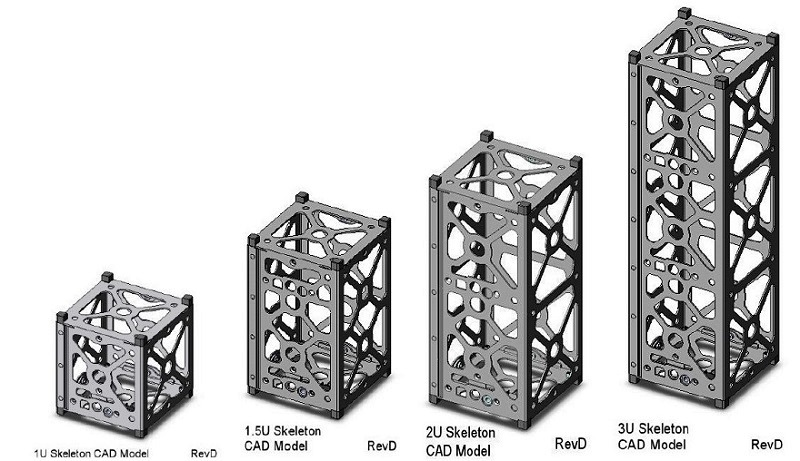
\includegraphics[width=0.75\textwidth]{CubesatConfig}}
\caption{Example of CubeSat Configurations\cite{configimage}}
\label{config}
\end{figure}

CubeSats that meet dimension and mass requirements can be launched from the Poly Picosatellite Orbital Deployer (P-POD) developed by Cal Poly.  The P-POD serves as a standardized deployment system for up to three 1U CubeSats or any equivalent combination.  Any CubeSat being deployed from a P-POD must adhere to additional specific guidelines in the CubeSat Design Specifications document in order to ensure compatibility for a successful deployment.  Some recently proposed experiments, however, have been designed for 6U CubeSat structures, resulting in the need for an alternative deployer.  Fortunately, NASA Wallops, NASA Ames, as well as other institutions have come up with designs for 6U deployers, all of which have been tested and have received a TRL of at least 6 \cite{SmSCTech}.

The standards developed by Cal Poly have resulted in a significant increase in the number of small satellite missions launched over the past few years \cite{MarketAssessment}.  This is partially due to the development of commercial off-the-shelf (COTS) components specifically designed to meet all CubeSat requirements.  Because of this, CubeSats have become relatively inexpensive, making them ideal educational tools in university and classroom settings.  With the development of COTS components, there are a variety of options for various processors and operating systems; however, these options may not always meet the criteria required for various missions.  It is for this reason that NASA IV\&V has been asked to develop a portable, pure software build-and-test system that will provide the capability to develop, debug, and test software on a standard personal computer with no specialized hardware.  Once this is developed, it is expected to be used in collaboration with NASA GSFC's SpaceCube development and testing. 

\section{Results of Survey}
To determine possible options for a standardized NASA IV\&V software, a comprehensive survey was conducted on past, present, and future CubeSat missions.  This survey initially consisted of all CubeSat missions able to be found online and totaled slightly over 250 missions.  For this particular report, it was decided that the focus would be on domestic missions which narrowed the search to approximately 150 missions, some of which had been launched while others were still only proposed concepts.  This list was consolidated once more to focus on already launched missions as well as those with launch services confirmed in upcoming years.  As a result, a comprehensive list of approximately 115 CubeSats has been developed.  The information included in this survey is summarized below in Table \ref{summary}.  This section of the report will provide a summary of data collected as a result of the survey.  

\begin{table}[h]
\centering
\caption{Summary of Data Collected for CubeSat Survey}
\label{summary}
\begin{tabular}{|l|l|l|}
\hline
\textbf{Mission Information} & \textbf{Launch Information} & \textbf{IV\&V Information} \\ \hline
Name of Satellite & Launch Date & Processor \\ \hline
Mission Objective & Launch Vehicle/Mission & Orbit \\ \hline
Sponsor & Mission Status & Uplink/Downlink \\ \hline
Manufacturer & Deployer & Attitude Determination \\ \hline
Domestic & Program & Attitude Control \\ \hline
Size & Orbit Parameters & Orbit Determination \\ \hline
Mass &  & Miscellaneous \\ \hline
\end{tabular}
\end{table}
A market assessment conducted by SpaceWorks Enterprises, Inc. in 2014 showed that of the nanosatellites launched between 2009 and 2013, 47\% can be categorized as 1U CubeSats.  Although not enough information is given to determine how many 2U and 3U CubeSats have been launched, it can be reasonably assumed that approximately 75\% of nanosatellites launched in that time frame can be considered CubeSats.  This high percentage shows just how popular CubeSats have become and gives reason to believe this number will continue to increase in the near future.  Based on the data collected in this survey, it can be confirmed that there has been a significant increase in the number of CubeSats launched per year as well as a migration towards 3U CubeSats (see Figure \ref{peryear}). 

\begin{figure}[h]
\centering
\frame{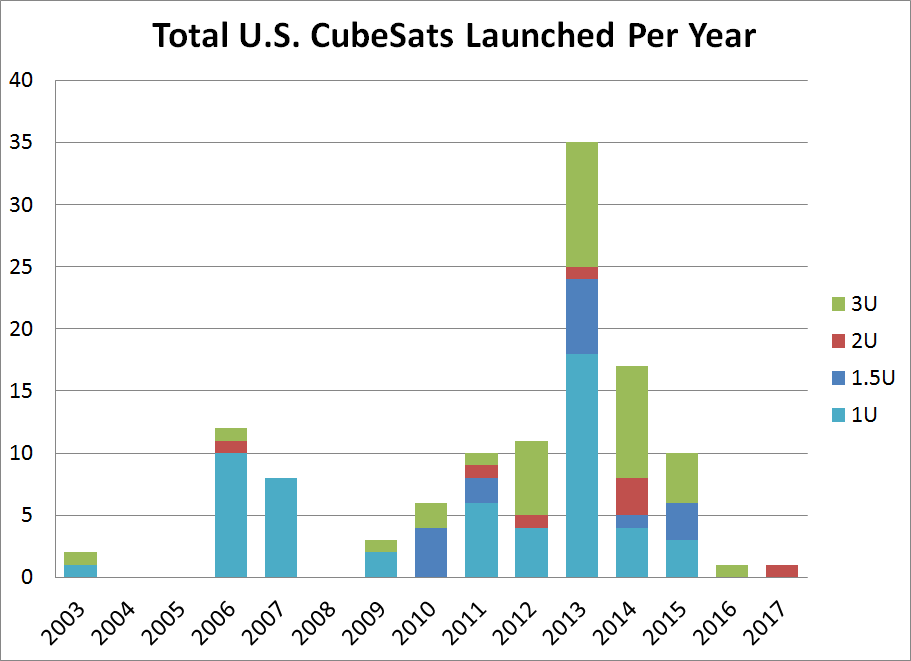
\includegraphics[width=0.75\textwidth,trim=0.1in 0.1in 0.1in 0.1in,clip]{Bar_SizeYear}}
\caption{Results of survey showing the size and number of CubeSats launched per year as of August 2014 (based on 116 CubeSats with applicable data)}
\label{peryear}
\end{figure}

Figure \ref{classperyear} shows the number of U.S. CubeSats launched per year based on class (i.e. private, civilian government, university, military, etc.).  It is obvious that a majority of launches have been for University missions and educational purposes.  However, there has been a significant increase seen in civilian government missions as well as privately funded missions.  

\begin{figure}[t!]
\centering
\frame{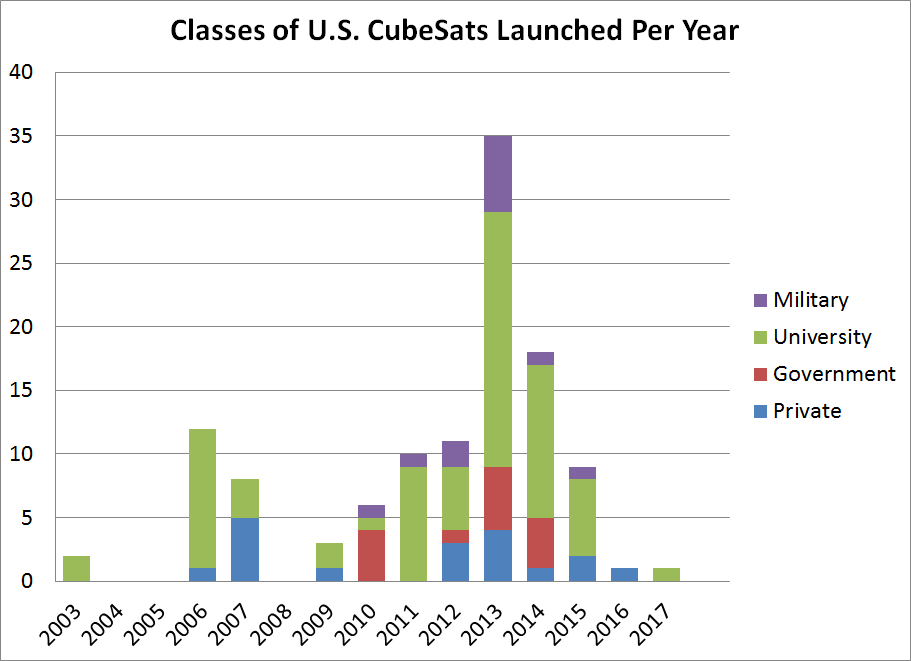
\includegraphics[width=0.75\textwidth,trim=0.1in 0.1in 0.1in 0.1in,clip]{Bar_Classes}}
\caption{Results of survey showing the number of U.S. CubeSats launched per year, divided by class, as of August 2014 (based on 116 CubeSats with applicable data)}
\label{classperyear}
\end{figure}

When considering verification and validation software, it is of most importance to determine the processor and operating system used for as many CubeSat missions as possible.  This will provide insight into which processors are most effective and capable of ensuring successful mission operations.  Of the CubeSats surveyed, almost 40\% used PIC processors.  Of these processors, 50\% used the PIC18.  These results are summarized in Figure \ref{processors}.  In addition, it should be noted that of these processors, TBC...

\begin{figure}[h!]
    \centering
    \begin{subfigure}[t]{0.5\textwidth}
        \centering
        \frame{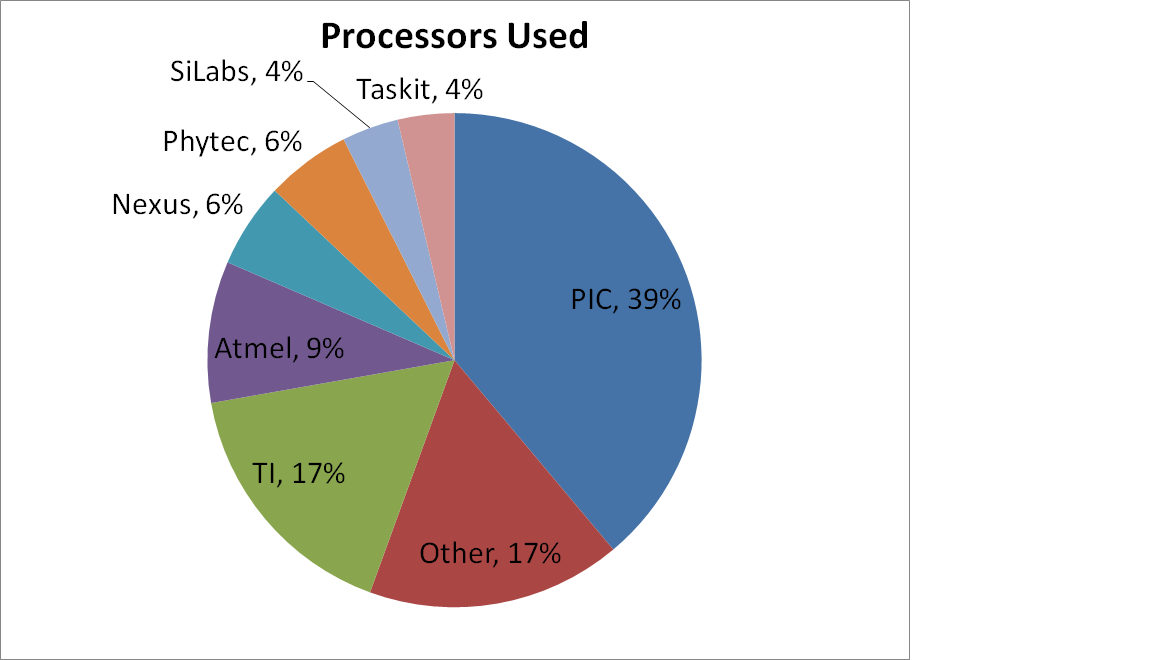
\includegraphics[height=2in,trim=0.1in 0.1in 0.1in 0.1in,clip]{Pie_Processors}}
        \caption{Summary of all processors used}
    \end{subfigure}%
    ~ 
    \begin{subfigure}[t]{0.5\textwidth}
        \centering
        \frame{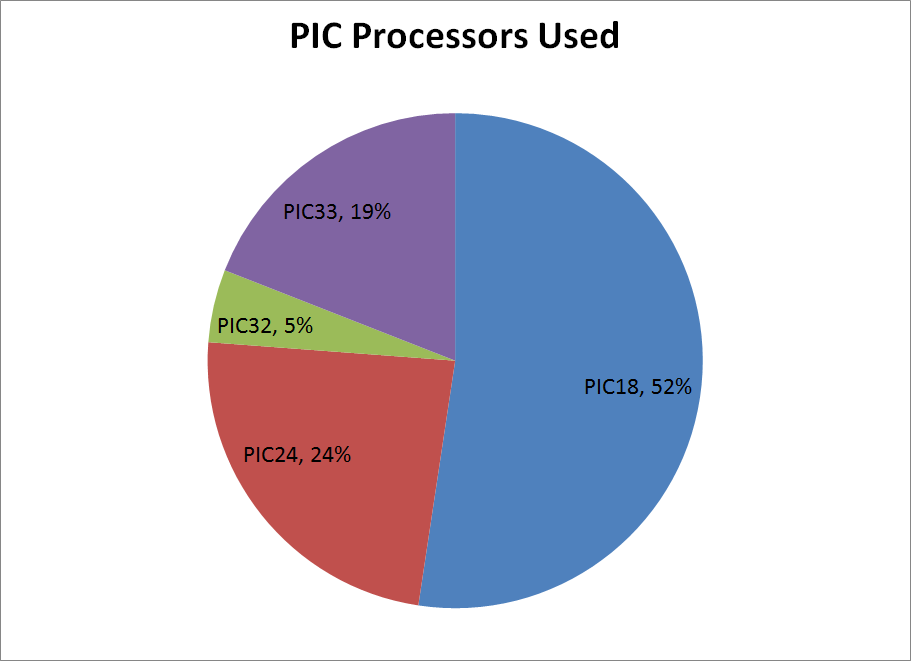
\includegraphics[height=2in,trim=0.1in 0.1in 0.1in 0.1in,clip]{Pie_PIC}}
        \caption{Breakdown of PIC processors used}
    \end{subfigure}
    \caption{Summary of processors used in CubeSats}
		\label{processors}
\end{figure}

As far as operating systems are concerned, Salvo and Linux were the two most commonly used in the CubeSat missions surveyed.  Salvo is available with the purchase of any Pumpkin Pluggable Processor Modules (PPM).


\begin{figure}[ht!]
\centering
\frame{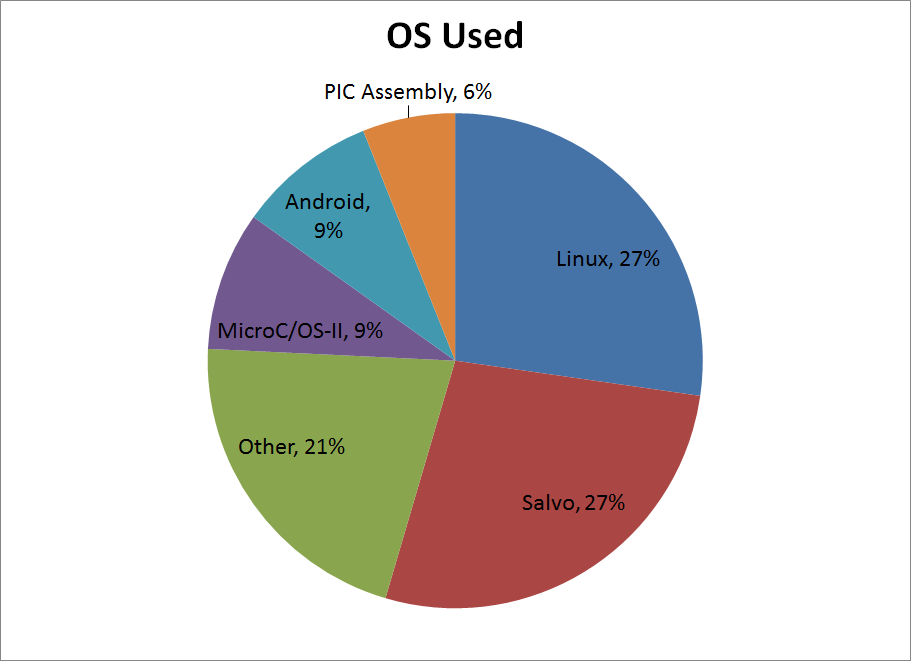
\includegraphics[width=0.75\textwidth,trim=0.1in 0.1in 0.1in 0.1in,clip]{Pie_OS}}
\caption{Results of survey showing the percentage of OS used in CubeSat missions}
\label{OS}
\end{figure}

\section{Discussion of Results}
................
\section{Future Work}
................

\bibliographystyle{aiaa}
\bibliography{CubeSatReferences}

\end{document}
